\title{
	DS-GS 1011 Assignment 1\\
	Bag of N-gram Document Classification
}
\author{
        Wenting Qi     \quad NetID: wq244\\
}

\documentclass[10pt]{article}
\usepackage[a4paper, total={7in, 11in}]{geometry}
\usepackage{graphicx}
\graphicspath{ {./Assignment1_Image/} }
\usepackage[font=scriptsize]{caption}
\usepackage{mwe}
\usepackage{wrapfig}
\usepackage[export]{adjustbox}
\usepackage{hyperref}

\begin{document}
\maketitle

\begin{abstract}
This paper explores the sentiment classification using the Standford AI database of the IMDB movie reviews. After building the basic Bag-of-Words model, the paper tunes different hyperparameters of the model, including the tokenization schemes, gram of words, vocabulary size, embedding size, type of optimizers, learning rate, number of epochs and batch sizes. The paper determines the performance of models basing on the accuracy rate shown on the validation data set and analyse influence of various hyperparameter to the model accordingly.
\end{abstract}

\section{Bag of Mono-gram Model}
In this section, the paper descibes how the baseline model is built starting form the data preperation, tokenizationa and word embedding.  Starting from building a model using the stochastic gradient descending optimizer, and gradually tuning different hyperparameters to improve the model.

\paragraph{Baseline Model}
To begin, the paper split the loaded data from train folder into two mutually exclusive data sets of training set and validation set of ratio 4:1. The model inputs are the reviews from IMDB and the targets are the labelled sentiment, positive or negative, for each review.  The paper aims to build a binary classification model through word embedding. All review data are tokenized using spacy English tokenizer and cleaned to be all lowercase and no punctuation for further use. The vocabulary is built from the top 10k most frequent tokens all the tokens from the training data set. The input words are transformed to indices through table looking. The words not in the vocabulary will be matched to 'unknown' with index 1.  All input are padded to the same length with 'pad' with index 0.\par
After the preperation, the next step would be model building. The paper start from the baseline model with word embedding dimension of 100, 3 mini-batches, stochastic gradient descending optimizer, and learning rate of 0.01 [Model I].

\paragraph{Learning Rate}
The first training for our baseline model gives a validation accuracy of 61.38\%  with highest accuracy rate of 62.72\%  at the first validation check of the 5th epoch. The accuracy rate show a steady but slow increase through training. It is suspected that the low learning rate is the reason of the slow imporvement. The paper heightens the learning rate to 0.10 [Model II] and 0.20 [Model III] and plot the training curves for the three models in Figure 1 below. \par
From the Figure 1, when learning rate rise to 0.10 and  0.20, the model soon reaches same level of accuracy as previous model at epoch 2 and still impoving afterwards. However the setbacks for the accuracy rate are severe too. As the learning rate gets higher, the parameter keep missing the minimum for the loss function by bouncing back and forth.\par
\begin{figure}[h]
\centering
\begin{minipage}{.4\textwidth}
  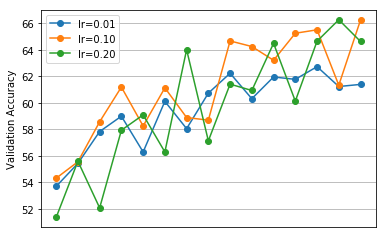
\includegraphics[width=\textwidth]{plot1}
  \caption{Training Curve of 5 Epochs for Various Learning Rate}
\end{minipage}%
\hfill
\begin{minipage}{.4\textwidth}
  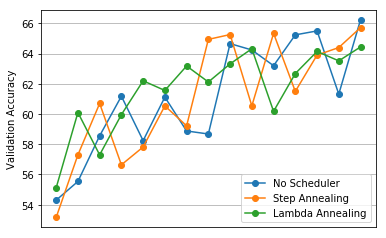
\includegraphics[width=\textwidth]{plot2}
  \caption{Training Curve of 5 Epochs with Learning Rate Scheduler}
\end{minipage}
\end{figure}
The more optimal learning rate would be the one that anneals gradually through the training. The paper applies learning rate step scheduler [Model IV] and lambda scheduler [Model V] to achieve the goal. The step scheduler is set to have the learning rate 0.1 for epoch 1-3, and learning rate \(0.1*0.8\) for epoch 3-5. The lambda scheduler is set to have \(0.8 ^ n\), where n is the number of epoch. The result gtraining curve is plot to Figure 2. Figure 2 shows that, by applying learning rate scheduler, the accuracy tend to stablize as the epoch number increases. The training curve with lambda scheduler behaves smoother at large epoch numbers. Thus, this paper would apply lambda scheduler for all later models.

 
\paragraph{Optimizer}
\begin{wrapfigure}{r}{0.4\textwidth} 

   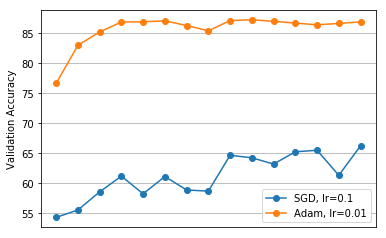
\includegraphics[width=0.4\textwidth,right]{plot3}
   \caption{Training Curve of 5 Epochs for Various Optimizer}

\end{wrapfigure} 
Though model with larger learning rate with scheduler gives higher accuracy of 64\%, the model performance is still far from satisfying. It is suspected that the model stuck at some small local minimum or plateu of the loss function. To overcome the local minimum, momentum 
needs to be introduced. The paper applies Adam optimizer to build a new model [Model VI]. \par
Figure 3 shows how significant the performance of model has been improved using Adam optimizer comparing to SGD optimizer. The Adam optimizer use the dacaying average of past gradient to create momentum thus improves the model. Notice the learning rate for model with Adam optimizer is set to 0.01 instead of 0.1, which performs best for SGD model., as model with Adam optimizer train quicker than SGD model. Learning rate of 0.1 will be too large, causing the accuracy to set back. The validation accuracy for current model reaches 87\%. The paper would keep applying Adam optimizer for later models.


\paragraph{Vocabulary Size and Embedding Dimension}
\begin{wrapfigure}{r}{0.4\textwidth} \

   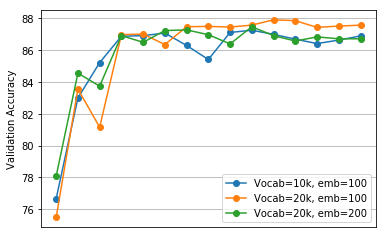
\includegraphics[width=0.4\textwidth,right]{plot4}
   \caption{Training Curve of 5 Epochs for Various Vocab Size and Emb Dim}

\end{wrapfigure} 
The current model performs fine, but this paper wishes to explore if by increasing the vocabulary size can further improve the model. The input are re-indixed due to the new vocabulary of size 20k and the new model [Model VII] is trained with the same hyperparameter as previous model. Figure 4 shows that with larger vocabulary, the validation accuracy for the model improves by 0.5\%. \par
Increasing the vocabulary size without increasing the embedding dimension accordingly might cause information loss through the process. Therefore, the paper tests for doubling the embedding dimension [Model VIII] and plot the result together on Figure 4. The training curve for model with embedding dimension 200 show a spike at the begining but fail to outperform later. Increasing the embedding dimension causes the irregularity of the surface to increase, thus harder to find minimum point even with the learning rate schedular. The end part of the training curve shows more instability comparing with the curve for dimension 100.


\paragraph{Tokenization Scheme}
\begin{wrapfigure}{r}{0.4\textwidth} 

   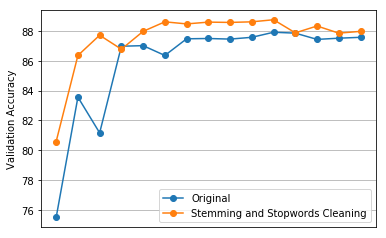
\includegraphics[width=0.4\textwidth,right]{plot5}
   \caption{Training Curve of 5 Epochs for Various Tokenization Scheme}

\end{wrapfigure} 
Pulling out the first few words from the vocabulary, there are many stopwords such as 'the', 'a', etc. These words are useless in our training to predict the sentiment of the review. Reading some review samples, it is found that there are some frequent words not included in the vocab becuase they are at different tenses. The current tokenization could be improved through stemming the words and removing the stopwords. In order to do so, the nltk stem and corpus packages are used. The new data set indexed using the new tokenization scheme of 20K-vocabulary is used to train the new model [Model IX]. Figure 5 shows that the new model has higher performance until the last epoch when the model starts to overfit the training set. By applying early stopping, the new model would have validation accuracy of 88.7\%. The paper will apply the new tokenization scheme for later models.

 


\section{Bag of Bi-gram Model}
This section, the model is trained through input tokens of two adjacent words instead of single-word tokens. By increasing the number of words in a single token, the model starts to take in account of the relationship between words, their orders and meaning of word groups.

\paragraph{Vocabulary Size and Embedding Dimension}
The bi-gram model is trained using vocabulary of size 10K [Model X], 20K [Model XI] and 40K [Model XII]. Figure 6 shows the model with larger vocabulary size have higher performance than the one trained using smaller vocabulary. Comparing with the two mono-gram model [Figure 4] of [Model VI] and [Model VII], the increase in vocabulary size shows more significant improvement in the model performance for the bi-gram model.\par
For large vocabulary size 40K, the embedding dimension is increased to 200 [Model XIII] and 300 [Model XIV] to see whether the model can be improved. Figure 7 shows that the increase of embedding dimension has little influence on the behavior of the model, yet the training time rises significantly as shown in Table 1.  To conclude, for bi-gram model, the [Model XII] with 40K vocabulary size and 100 embedding dimension is the optimal choice.

\begin{table}[h]
\centering
\caption{Training Time for Various Embedding Dimensions}
\label{my-label}
\begin{tabular}{lll}
\hline
                        & Validation Accuracy & Training Time \\ \hline
Embedding Dimension 100 & 85.40\%             & 105.58s       \\
Embedding Dimension 200 & 85.04\%             & 174.55s       \\
Embedding Dimension 300 & 85.18\%             & 243.00s       \\ \hline
\end{tabular}
\end{table}

\begin{figure}[h]
\centering
\begin{minipage}{.4\textwidth}
  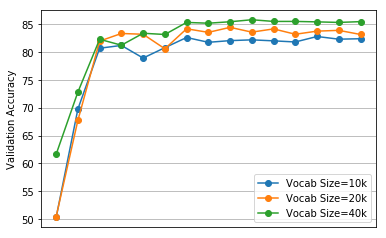
\includegraphics[width=\textwidth]{plot6}
  \caption{Bi-gram Model Training Curve of 5 Epochs for Various Vocab Size}
\end{minipage}%
\hfill
\begin{minipage}{.4\textwidth}
  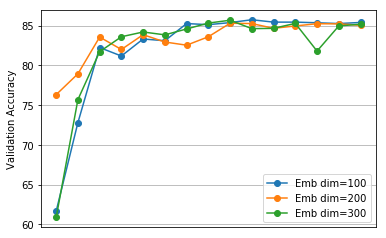
\includegraphics[width=\textwidth]{plot7}
  \caption{Bi-gram Model Training Curve of 5 Epochs with Embedding Dimension}
\end{minipage}
\end{figure}



\section{Bag of Tri-gram Model}
\begin{figure}[h]
\centering
\begin{minipage}{.4\textwidth}
  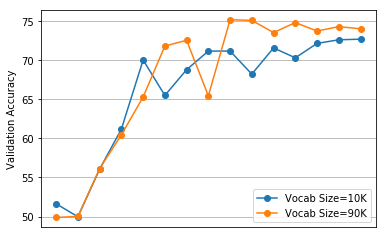
\includegraphics[width=\textwidth]{plot8}
  \caption{Tri-gram Model Training Curve of 5 Epochs for Various Vocab Size}
\end{minipage}%
\hfill
\begin{minipage}{.4\textwidth}
  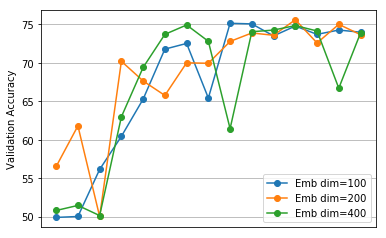
\includegraphics[width=\textwidth]{plot9}
  \caption{Tri-gram Model Training Curve of 5 Epochs with Various Embedding Dimension}
\end{minipage}
\end{figure}
This section, the model is trained through input tokens of three adjacent words. As the number of word gram increases, the total number of distinct tokens increases exponentialy.  The paper explores larger vocabulary size and embedding dimension. Noticed as the embedding dimension increases, the irregularity increases. This section tries to alter the batch size to help with the surface irregularity problem.


\begin{wrapfigure}{r}{0.4\textwidth} 

   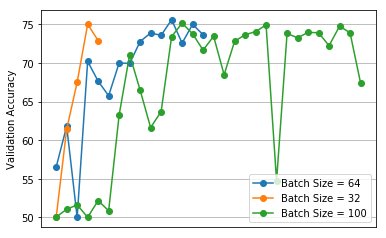
\includegraphics[width=0.4\textwidth,right]{plot10}
   \caption{Tri-gram Training Curve of 5 Epochs for Various Batch Size}

\end{wrapfigure} 
\paragraph{Vocabulary Size and Embedding Dimension}

Since the number of word gram increases, the combination or words increases exponentially. The paper explores large vocabulary size of \(3^2 * 10K\). The tri-gram model is trained using vocabulary size of 10K [Model XIII] and 90K [Model XIV]. Figure 8 shows, the large vocabulary size has trivial improvement on the model performance. \par


It is suspected that the small embedding dimension may cause the loss of information during the transform. Thus, new model is trained with embedding dimension of 200 [Model XV] and 300 [Model XVI]. Figure 9 shows the increase in embedding size fail to outperform. Larger embedding size enables the model to reach better performance earlier than smaller embedding size, yet the performance is more unstable during the training.



\paragraph{Batch Size}
The new model is trained with batch size of 100 [Model XVII] and 32 [Model XVIII]. Figure 10 shows the batch size fail to improve the model performance. Therefore, for tri-gram model, [Model XVII] with 90K vocabulary, 200 embedding size and 100 batch size is the optimal.

\begin{wrapfigure}{r}{0.4\textwidth} 

   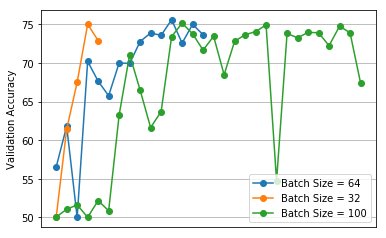
\includegraphics[width=0.4\textwidth,right]{plot10}
   \caption{Tri-gram Training Curve of 5 Epochs for Various Batch Size}

\end{wrapfigure} 

\section{Bag of Quad-gram Model}
This section will start with the basic quad-gram model of vocabulary size 10k embedding dimension of 100, and use the tuning knowledge from above to tune the model to gain higher validation accuracy. \par
The different best N-gram models will be compared for their performances to choose the final model.

\paragraph{Vocabulary Size}
The Quad-gram model is trained with vocabulary size of 10K [Model XIX] and 160K [Model XX].   Figure 11 shows that the vocabulary size has trivial improvement on the model performance. It is suspected that the amount of training data is insufficient with respect to the large vocabulary.

\paragraph{Batch Size}
The model is trained with batch size of 100 [Model XXI] and 32 [Model XXII]. 
Figure 12 shows the batch size does not influence much on the performance of the model yet smaller batch size gives less updates on the parameter.  Table 2 shows the large batch size model doubles the training time which is highly inefficient.


\begin{figure}[h]
\centering
\begin{minipage}{.4\textwidth}
  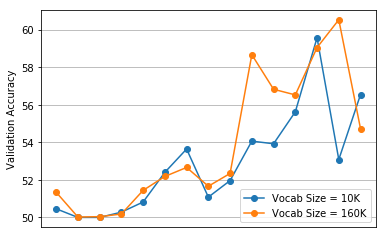
\includegraphics[width=\textwidth]{plot11}
  \caption{Quad-gram Model Training Curve of 5 Epochs for Various Vocab Size}
\end{minipage}%
\hfill
\begin{minipage}{.4\textwidth}
  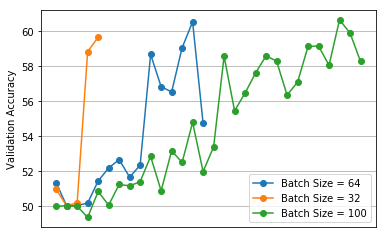
\includegraphics[width=\textwidth]{plot12}
  \caption{Quad-gram Model Training Curve of 5 Epochs with Various Batch Size}
\end{minipage}
\end{figure}


\begin{table}[h]
\centering
\caption{Training Time of Quad-gram Model with Various Batch Size}
\label{my-label}
\begin{tabular}{llllll}
\hline
                                & Vocabulary Size & Embedding Size & Batch Size & Validation Accuracy & Training Time \\ \hline
\multicolumn{1}{l|}{Model XX}   & 160K            & 400            & 64         & 54.72\%             & 1166.21s        \\
\multicolumn{1}{l|}{Model XXI}  & 160K            & 400            & 100        & 59.64\%             & 174.55s       \\
\multicolumn{1}{l|}{Model XXII} & 160K            & 400            & 32         & 58.26\%             & 3885.92s      \\ \hline
\end{tabular}
\end{table}

\paragraph{Compare between N-gram Models}
From  Table 3, we can clearly see that the Bag of Words [Model IV] has the best performance and standable training hours. The three correct predictions and three incorrect predictions are shown in Table 4 at the next page. The paper deploy the model on test set and gives the accuracy rate of \textbf{86.044\%}.
\begin{table}[h]
\caption{Performance Comparison between N-gram Models}
\label{my-label}
\resizebox{\textwidth}{!}{%
\begin{tabular}{lllllll}
\hline
                                & Vocabulary Size & Embedding Size & Batch Size & Number of Epoch & Validation Accuracy & Training Time \\ \hline
\multicolumn{1}{l|}{Model IV}   & 20000           & 100            & 64         & 5               & 88.70\%             & 92.74s        \\
\multicolumn{1}{l|}{Model XII}  & 40000           & 100            & 64         & 5               & 85.40\%             & 105.58s       \\
\multicolumn{1}{l|}{Model XVII} & 90000           & 200            & 100        & 5               & 72.9\%              & 243.00s       \\
\multicolumn{1}{l|}{Model XIX}  & 10000           & 100            & 64         & 5               & 56.54\%             & 74.06s        \\ \hline
\end{tabular}%
}
\end{table}

\begin{table}[t]
\caption{Correct and Incorrect Prediction Samples}
\centering
\label{my-label}
\resizebox{\textwidth}{!}{%
\begin{tabular}{lll|lll}
\multicolumn{3}{l|}{Three Incorrect Prediction} & \multicolumn{3}{l}{Three Correct Prediction} \\ \hline
Indices Data      & Label     & Predicted     & Indices Data      & Label      & Predicted     \\ \hline
3281, 593, 12220, 149...  & 1       & 0              & 169, 4, 873, 222, 14...                  &0            &0               \\
26, 54, 223, 485, 260...        & 0       & 1              & 1543, 751, 77, 659...                  &1            &1               \\
 2289, 295, 916, 288...        & 1       & 0              &32, 4, 111, 6, 12...                   &1            &1              
\end{tabular}%
}
\end{table}

\section{Bonus}
The paper extract the score target from the file name and try using the bag of word model with Adam optimizer [Model XXII] to train. The paper explores half the batch size [Model XXIV], doubling vocab size [Model XXV], adding more layer to the model [Model XXVI], using bi-gram model to take in account of word groups [Model XXVII]. The performance all remain around 40\%. It is suspected that the maximum sentence length and training data size might be the hyperparameters worth further exploration.

\section{Appendix}

All the python code are uploaded to github as jupyter notebook file at the following link:
\url{https://github.com/nicoleqiwt/NLP_1011.git}

\end{document}
